% IEEE-format paper. Build from the project root:
%   docker run --rm -v "${PWD}:/w" -w /w/docs texlive/texlive pdflatex REPORT_IEEE.tex   (run twice)
% All reported numbers come from ../outputs/metrics/. Figures are the charts in ../outputs/charts/.
\documentclass[10pt,journal]{IEEEtran}
\usepackage[utf8]{inputenc}
\usepackage[T1]{fontenc}
\usepackage{graphicx}
\usepackage{amsmath}
\usepackage{booktabs}
\usepackage{url}
\usepackage{tikz}
\usetikzlibrary{arrows.meta,positioning,shapes.geometric,fit}
\usepackage{cite}
\graphicspath{{../outputs/charts/}}
\hyphenation{Spark Kafka Hadoop co-occurrence}

\tikzset{
  box/.style={draw,rounded corners=1pt,align=center,minimum height=0.62cm,font=\fontsize{6.5}{7.5}\selectfont,inner sep=2pt,fill=blue!8},
  store/.style={box,fill=orange!15},
  proc/.style={box,fill=green!12},
  arr/.style={-{Stealth[length=1.6mm]},thick}
}

\begin{document}

\title{Session-Aware Real-Time Recommendation over E-Commerce Clickstreams: ALS Fold-In with Kafka and Spark Structured Streaming on a Resource-Constrained Hadoop Cluster}

\author{Kirupashankar Chockkanathan, Padmacharan R, Prapanjan I, and Shree Santh B\\
Amrita School of Artificial Intelligence, Amrita Vishwa Vidyapeetham%
\thanks{Source code, metrics and charts: \protect\url{https://github.com/kirupashankarchockkanathan/Clickstream-Recommender}.}}

\markboth{Session-Aware Recommendation with ALS Fold-In over Kafka and Spark}{}
\maketitle

\begin{abstract}
Session-based recommendation must react to the clicks of an ongoing visit, often for anonymous users, while event volumes exceed a single machine. This paper presents a distributed streaming implementation of alternating-least-squares (ALS) \emph{fold-in}, which re-solves a session vector from the clicks observed so far without retraining the model, built on Apache Kafka, Spark Structured Streaming and a Hadoop cluster (one NameNode, three DataNodes, replication 3) running on a single 16\,GB machine. The platform is evaluated on 109.95 million real click events (26.3\,GiB as JSON Lines) and five relational tables, with a strict temporal split and 159{,}629 held-out next-item cases. Fold-in improves hit rate at 20 from 0.132 (stale batch ALS) to 0.370 after one click, a factor of 2.8, and costs about 6\,ms per request. An item co-occurrence baseline remains the strongest single method (0.440), and a rank-fusion hybrid is best only at the first click (0.454). The streaming pipeline delivers recommendations with a median click-to-result latency of 8.5\,s. Measured storage, partitioning and caching trade-offs are reported.
\end{abstract}

\begin{IEEEkeywords}
Recommender systems, session-based recommendation, alternating least squares, Apache Spark, Apache Kafka, Hadoop, structured streaming, clickstream.
\end{IEEEkeywords}

\section{Introduction}
\IEEEPARstart{I}{n} e-commerce, a large share of visitors are anonymous or new, so recommendations increasingly rely on the short-term intent visible in the clicks of the current session rather than on a long-term profile \cite{wang2021survey,ludewig2021}. Serving such recommendations at scale requires an architecture that ingests a continuous event stream, keeps per-session state and combines it with models trained offline on large histories. Latent-factor models such as ALS capture collaborative structure well but are trained in batch, so their user representations become stale as soon as the visitor continues to click.

\textbf{Research gap.} Session-based algorithms are predominantly compared through single-machine offline replay \cite{ludewig2021,wang2021survey}. Spark-based ALS has been studied \cite{li2020als,kumar2021edmfals}, and streaming matrix factorization has been proposed independently of Spark ALS \cite{jakomin2020simf}. To the best of the authors' knowledge, no journal study evaluates session-aware ALS inside Spark Structured Streaming over Kafka on a Hadoop cluster against item-based baselines under a leakage-free temporal protocol \cite{ji2023leakage}.

\textbf{Contributions.}
\begin{enumerate}
\item A distributed Scala implementation of ALS fold-in for sessions, usable both in batch evaluation and inside a Structured Streaming job.
\item A temporal evaluation of five recommenders (popularity, batch ALS, ALS fold-in, item co-occurrence and a hybrid) on 110\,M real click events.
\item A measured Kafka--Spark--Kafka latency and a set of storage and execution-tuning measurements, including those that did not help.
\end{enumerate}

\section{Related Work}
Table~\ref{tab:lit} summarises the journal literature on which the work builds.

\begin{table}[!t]
\caption{Journal literature used}
\label{tab:lit}
\centering
\footnotesize
\begin{tabular}{@{}p{0.5cm}p{5.2cm}p{2.1cm}@{}}
\hline
\textbf{Ref.} & \textbf{Topic} & \textbf{Venue, year}\\\hline
\cite{ludewig2021} & Twelve session-based algorithms compared; kNN heuristics often preferable & UMUAI, 2021\\
\cite{wang2021survey} & Survey and taxonomy of session-based recommenders & ACM CSUR, 2021\\
\cite{jakomin2020simf} & Incremental matrix factorization fusing several data streams (Yelp) & ESWA, 2020\\
\cite{vinagre2021eval} & Prequential k-fold evaluation with online significance tests & IEEE TKDE, 2021\\
\cite{ji2023leakage} & Data leakage when splits ignore the global timeline & ACM TOIS, 2023\\
\cite{raptis2023kafka} & Survey of research on Apache Kafka for data streaming & IEEE Access, 2023\\
\cite{zaharia2016spark} & Spark as a unified engine for batch and streaming & CACM, 2016\\
\cite{li2020als} & ALS collaborative filtering for MovieLens on Hadoop and Spark & IJGUC, 2020\\
\cite{kumar2021edmfals} & Distributed matrix-factorization ALS on Spark & JIKM, 2021\\\hline
\end{tabular}
\end{table}

\textbf{Session-based recommendation.} Wang \emph{et al.} \cite{wang2021survey} give a problem statement and taxonomy of session-based recommenders, which distinguishes short-term, dynamic preference from the long-term static preference modelled by classical collaborative filtering. Ludewig \emph{et al.} \cite{ludewig2021} compare twelve algorithms, six of them neural, under identical conditions and report that the accuracy gains of neural methods are limited and that nearest-neighbour heuristics are in most cases preferable. Their experiments are offline and single-machine. The present work adopts this question and moves it to a distributed streaming setting with a latent-factor method (ALS fold-in) in addition to a neighbour-style baseline; neural models and the full SKNN family are not included, and absolute numbers are not compared with \cite{ludewig2021} because datasets, catalogues and protocols differ.

\textbf{Incremental and streaming models.} Jakomin \emph{et al.} \cite{jakomin2020simf} propose incremental matrix factorization that fuses multiple heterogeneous data streams and adapts to concept change. The present approach addresses staleness differently: item factors are kept fixed and only the session vector is re-solved in closed form, which requires no model update but also cannot adapt the item space. Vinagre \emph{et al.} \cite{vinagre2021eval} propose prequential evaluation with online significance tests for stream-based recommenders; this paper uses a temporal hold-out instead and leaves prequential testing to future work.

\textbf{Evaluation methodology.} Ji \emph{et al.} \cite{ji2023leakage} show that splits ignoring the global timeline leak future interactions and change model rankings; the protocol here splits strictly by time.

\textbf{Platforms.} Spark \cite{zaharia2016spark} provides batch and streaming execution on one engine, Kafka is the standard event log (see the survey in \cite{raptis2023kafka}), and Spark-based ALS has been studied on MovieLens \cite{li2020als} and as a distributed method \cite{kumar2021edmfals}. The present work uses a trained ALS model for session-level inference inside a streaming pipeline.

\section{System Architecture}
The platform runs in Docker on WSL2 (12\,GB of the machine's 15.7\,GB usable RAM, 8 logical processors). Table~\ref{tab:cluster} gives the specification, and Figs.~\ref{fig:arch} and~\ref{fig:flow} show the structure and the data flow. HDFS uses the default replication factor of 3 on three DataNodes; \texttt{fsck} reports 315 blocks with an average replication of 3.0 and no under-replicated blocks. All three DataNodes share one physical SSD, so replication exercises the mechanism but offers no hardware fault tolerance.

\begin{table}[!t]
\caption{Cluster specification (container memory caps; idle use about 3.5\,GB in total)}
\label{tab:cluster}
\centering
\footnotesize
\begin{tabular}{@{}llp{3.9cm}@{}}
\hline
\textbf{Component} & \textbf{Count} & \textbf{Memory cap / role}\\\hline
HDFS NameNode & 1 & 1.25\,GB (heap 768\,MB)\\
HDFS DataNode & 3 & 768\,MB each (heap 384\,MB), repl.\ 3\\
YARN ResourceManager & 1 & 768\,MB\\
YARN NodeManager & 1 & 4.5\,GB cap; 3.5\,GB and 6 vcores offered to jobs\\
Job HistoryServer & 1 & 512\,MB\\
Kafka 3.7 (KRaft) & 1 broker & 1\,GB, topics with 6 partitions\\
PostgreSQL 16 & 1 & 512\,MB\\
Spark 3.5.1 client (Java 8) & 1 & 2\,GB; executors 2$\times$1.25\,GB, 2 cores\\\hline
\end{tabular}
\end{table}

\begin{figure}[!t]
\centering
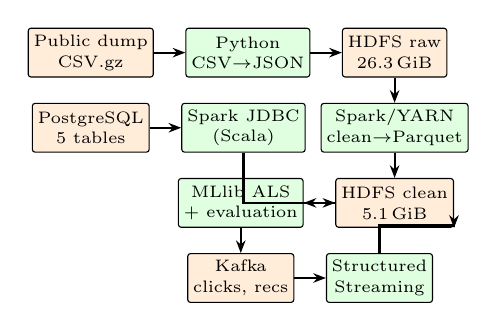
\begin{tikzpicture}[node distance=3.2mm and 4mm]
  \node[store] (src) {Public dump\\CSV.gz};
  \node[proc,right=of src] (conv) {Python\\CSV$\to$JSON};
  \node[store,right=of conv] (raw) {HDFS raw\\26.3\,GiB};
  \node[store,below=of src] (pg) {PostgreSQL\\5 tables};
  \node[proc,right=of pg] (jdbc) {Spark JDBC\\(Scala)};
  \node[proc,below=of raw] (etl) {Spark/YARN\\clean$\to$Parquet};
  \node[store,below=of etl] (clean) {HDFS clean\\5.1\,GiB};
  \node[proc,left=of clean] (als) {MLlib ALS\\+ evaluation};
  \node[store,below=of als] (kafka) {Kafka\\clicks, recs};
  \node[proc,right=of kafka] (ss) {Structured\\Streaming};
  \draw[arr] (src)--(conv); \draw[arr] (conv)--(raw); \draw[arr] (raw)--(etl);
  \draw[arr] (pg)--(jdbc); \draw[arr] (jdbc)|-(clean.west);
  \draw[arr] (etl)--(clean); \draw[arr] (clean)--(als); \draw[arr] (als)--(kafka);
  \draw[arr] (kafka)--(ss); \draw[arr] (ss.north) -- ++(0,0.35) -| (clean.south east);
\end{tikzpicture}
\caption{System architecture. Orange: storage; green: processing. The batch model is trained on HDFS data and then used by the streaming job reading Kafka.}
\label{fig:arch}
\end{figure}

\begin{figure*}[!t]
\centering
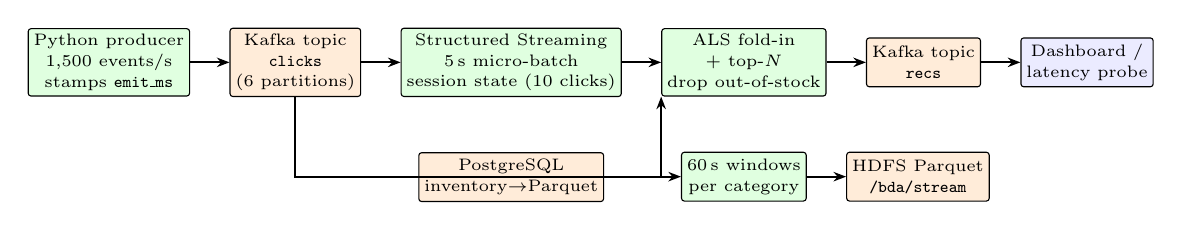
\begin{tikzpicture}[node distance=5mm]
  \node[proc] (prod) {Python producer\\1{,}500 events/s\\stamps \texttt{emit\_ms}};
  \node[store,right=of prod] (clicks) {Kafka topic\\\texttt{clicks}\\(6 partitions)};
  \node[proc,right=of clicks] (state) {Structured Streaming\\5\,s micro-batch\\session state (10 clicks)};
  \node[proc,right=of state] (fold) {ALS fold-in\\+ top-$N$\\drop out-of-stock};
  \node[store,right=of fold] (recs) {Kafka topic\\\texttt{recs}};
  \node[box,right=of recs] (dash) {Dashboard /\\latency probe};
  \node[proc,below=7mm of fold] (win) {60\,s windows\\per category};
  \node[store,right=of win] (hdfs) {HDFS Parquet\\\texttt{/bda/stream}};
  \node[store,below=7mm of state] (pgt) {PostgreSQL\\inventory$\to$Parquet};
  \draw[arr] (prod)--(clicks); \draw[arr] (clicks)--(state); \draw[arr] (state)--(fold); \draw[arr] (fold)--(recs); \draw[arr] (recs)--(dash);
  \draw[arr] (clicks) |- (win); \draw[arr] (win)--(hdfs); \draw[arr] (pgt)-|(fold.south west);
\end{tikzpicture}
\caption{Streaming data flow (Kafka $\to$ Spark $\to$ Kafka/HDFS). Latency is result time minus producer time.}
\label{fig:flow}
\end{figure*}

\section{Data}
\textbf{Source.} The clickstream is the REES46 e-commerce behaviour data set (Kaggle dataset \url{mkechinov/ecommerce-behavior-data-from-multi-category-store}), October and November 2019 \cite{kechinov}. Attributes are event time, event type (view, cart, remove\_from\_cart, purchase), product id, category id and code, brand, price, user id and user session. The files are distributed as compressed CSV and are converted to JSON Lines at ingestion, so that the clickstream is held as semi-structured data alongside relational tables.

\textbf{Volume and variety.} The data comprises 109{,}950{,}743 events, 26.3\,GiB as JSON Lines in 106 files (79\,GiB on disk with three replicas). Structured data is held in PostgreSQL: \texttt{products} (206{,}876 rows), \texttt{orders} (1{,}402{,}758), \texttt{order\_items} (1{,}659{,}788), \texttt{users} (5{,}316{,}649) and \texttt{inventory} (206{,}876).

\textbf{Velocity and veracity.} Velocity is generated by replaying recorded events through Kafka at a controlled rate (1{,}500 events/s). Veracity is handled by the cleaning stage in Section~\ref{sec:clean}.

\textbf{Real, synthetic and simulated components.} Table~\ref{tab:real} states the provenance of each component. User profiles and inventory levels are generated, so conclusions about their effect on recommendation quality cannot be drawn from this data.

\begin{table}[!t]
\caption{Provenance of data components}
\label{tab:real}
\centering
\footnotesize
\begin{tabular}{@{}lll@{}}
\hline
\textbf{Component} & \textbf{Status} & \textbf{Note}\\\hline
Click events & real & REES46, Oct--Nov 2019\\
products, orders, order\_items & real-derived & from the events\\
users (region, segment, signup) & \textbf{synthetic} & hash of user id\\
inventory (stock 0--499) & \textbf{synthetic} & hash of product id\\
Event rate through Kafka & \textbf{simulated} & replay of recorded events\\
User / session sample & sampled & 25\% users, 20\% test sessions\\\hline
\end{tabular}
\end{table}

\section{Methodology}
\subsection{Data Cleaning}\label{sec:clean}
A Scala/Spark job parses the JSON once into typed Parquet and then removes, with every stage counted, rows missing a key field, rows with an invalid event type, price $\le 0$ or null, exact duplicates, and sessions longer than 1{,}000 events (bot-like). Missing brand or category values are labelled ``unknown''. Of 109{,}950{,}743 rows, 402{,}558 (0.37\%) are removed: 12 with missing key fields, 256{,}761 with invalid prices, 130{,}646 duplicates and 15{,}139 rows in bot-like sessions. The cleaned data occupies 5.1\,GiB of Parquet, partitioned by day (Fig.~\ref{fig:veracity}).

\begin{figure}[!t]
\centering
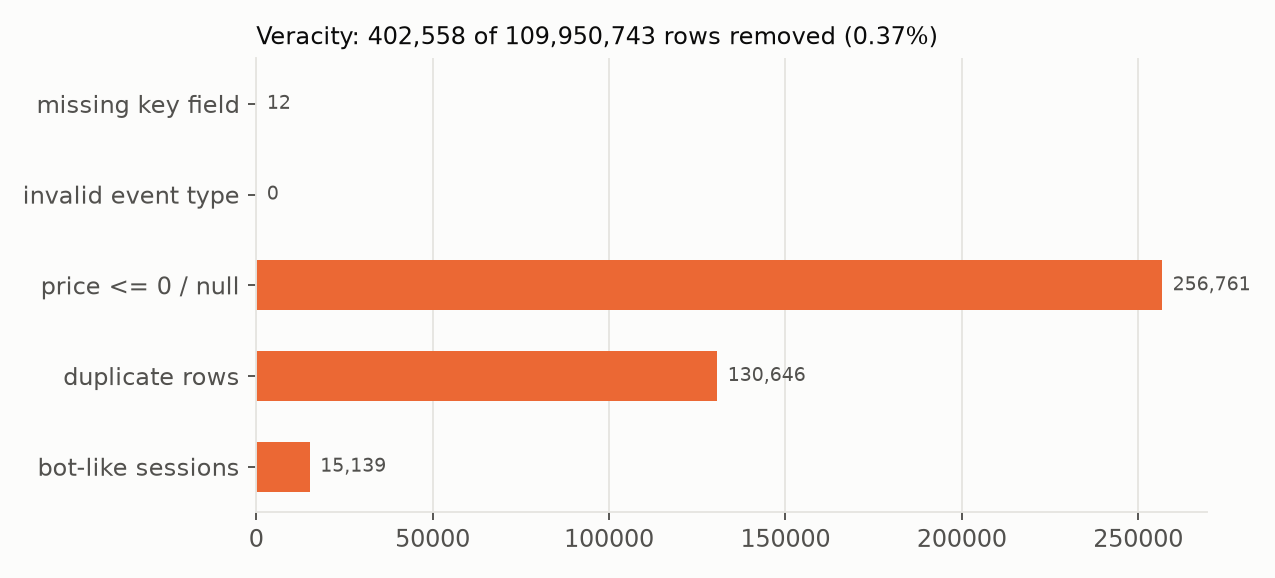
\includegraphics[width=0.85\columnwidth]{veracity.png}
\caption{Rows removed by each cleaning rule.}
\label{fig:veracity}
\end{figure}

\subsection{Recommenders}
Interaction strength is view\,=\,1, cart\,=\,3 and purchase\,=\,5, summed per (user, item). Five methods are compared.
\begin{enumerate}
\item \textbf{Popularity}: the most popular catalogue items in the training data.
\item \textbf{Batch ALS}: MLlib implicit ALS (rank 64, $\alpha=40$, $\lambda=0.05$, 8 iterations). The user vector is fixed at training time and ignores the current session; unseen users fall back to popularity.
\item \textbf{ALS fold-in}: with fixed item factors $Y$ and confidences $c_i=1+\alpha r_i$, the session vector solves
\begin{equation}
\Big(Y^{\top}Y+\sum_{i\in S}(c_i-1)\,y_iy_i^{\top}+\lambda|S|I\Big)x=\sum_{i\in S}c_i\,y_i ,
\end{equation}
implemented in Scala with a Cholesky solver; $Y^{\top}Y$ is computed once and broadcast.
\item \textbf{Item co-occurrence}: window 3, weights $1/\text{distance}$, normalised by $\sqrt{f_af_b}$, top-50 neighbours per item, and the last three clicks with decay 0.5.
\item \textbf{Hybrid}: reciprocal-rank fusion ($k=60$) of the fold-in and co-occurrence lists.
\end{enumerate}
Hyper-parameters are selected on a validation window (training to November 13, validation November 14--20, seven configurations) and never on the test window.

\subsection{Evaluation Protocol}
The evaluation uses a strict temporal split \cite{ji2023leakage}: training on events up to November 20 and test sessions from November 21 to 30. Users are a deterministic 25\% hash sample, and the catalogue consists of the 45{,}863 items with at least 30 distinct training users. For each sampled test session, the unique catalogue items in first-click order define cases consisting of a prefix of $k=1,2,3$ items and the next new item. Prefix weights use only the first event on each item, so later events cannot leak into the prefix. This yields 159{,}629 cases (77{,}772, 48{,}719 and 33{,}138 for $k=1,2,3$). Cases whose target lies outside the catalogue are removed, so results describe catalogue items only. Metrics are HR@20, MRR@20 and NDCG@20.

\subsection{Streaming Implementation}
A Python producer replays events into the Kafka topic \texttt{clicks} and stamps each with \texttt{emit\_ms}. A Scala Structured Streaming job with 5\,s micro-batches keeps the last ten clicks per session using \texttt{flatMapGroupsWithState} (30-minute timeout), computes the fold-in vector, selects the top ten items, removes out-of-stock items using the PostgreSQL-derived inventory table (413 items with zero stock) and writes JSON to the topic \texttt{recs}. A second query computes 60\,s windows sliding every 10\,s per category and writes them to HDFS. Latency is the result timestamp minus \texttt{emit\_ms}.

\subsection{Performance Tuning Experiments}
Six experiments (E1--E6) are run once each on the cluster: E1 JSON versus Parquet scans; E2 shuffle partitions (4, 24, 96, 400); E3 caching; E4 500 small files versus 8 files; E5 broadcast versus sort-merge join; E6 partition pruning. As each is a single run, differences below roughly 15\% are within noise.

\section{Results}
\subsection{Recommendation Accuracy}
Table~\ref{tab:results} and Fig.~\ref{fig:acc} give the test results.

\begin{table}[!t]
\caption{HR@20 / NDCG@20 on 159{,}629 test cases (best per column in bold)}
\label{tab:results}
\centering
\footnotesize
\begin{tabular}{@{}lccc@{}}
\hline
\textbf{Method} & \textbf{$k$=1} & \textbf{$k$=2} & \textbf{$k$=3}\\\hline
Popularity & 0.094 / 0.040 & 0.070 / 0.028 & 0.058 / 0.023\\
ALS batch (stale) & 0.132 / 0.057 & 0.105 / 0.043 & 0.087 / 0.035\\
ALS + fold-in & 0.370 / 0.177 & 0.335 / 0.151 & 0.293 / 0.126\\
Co-occurrence & 0.440 / 0.216 & \textbf{0.449} / \textbf{0.216} & \textbf{0.432} / \textbf{0.203}\\
Hybrid (RRF) & \textbf{0.454} / \textbf{0.223} & 0.445 / 0.208 & 0.418 / 0.188\\\hline
\end{tabular}
\end{table}

\begin{figure*}[!t]
\centering
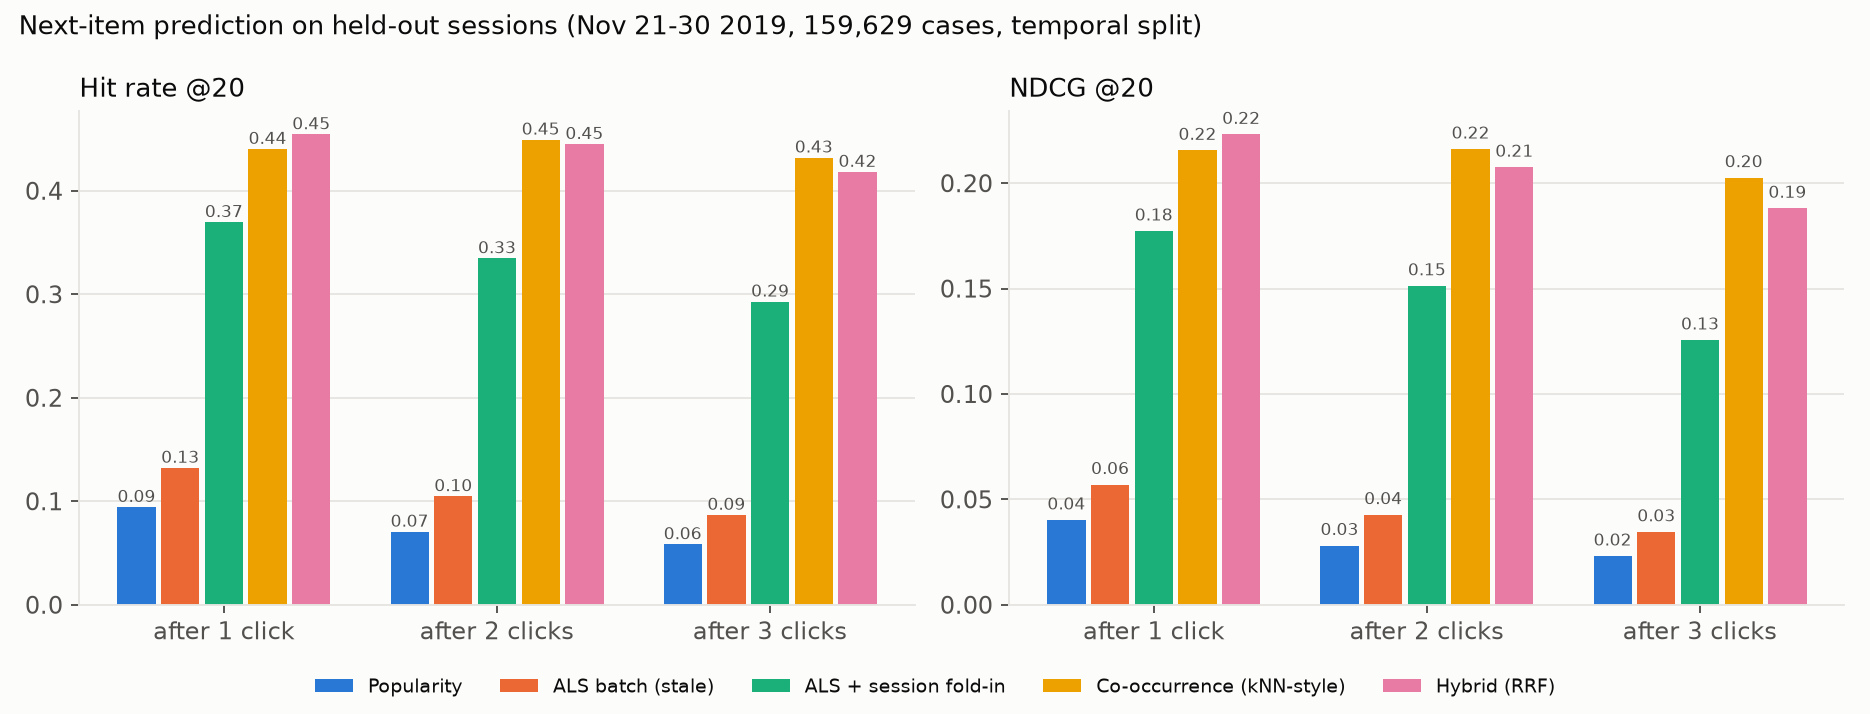
\includegraphics[width=0.78\textwidth]{eval_methods.png}
\caption{Hit rate and NDCG at 20 by prefix length for the five methods.}
\label{fig:acc}
\end{figure*}

Folding in the session raises HR@20 after one click from 0.132 for the stale batch vector to 0.370, a factor of 2.8. Item co-occurrence outperforms fold-in at every prefix length, and the hybrid is best only at $k=1$ (0.454 versus 0.440), a margin that the present single-run design cannot establish as significant. Fold-in accuracy declines with longer prefixes, whereas co-occurrence remains stable. On the validation window, higher ALS rank improves fold-in (NDCG@20 after one click: 0.142, 0.176, 0.205 and 0.228 for ranks 16, 32, 64 and 128), but rank 128 trains 4.5$\times$ slower (304\,s versus 67\,s) and serves 5.8\,ms instead of 2.3\,ms per request; rank 64 is therefore used. In the final run ALS training takes 355\,s, and one fold-in with top-20 selection over 45{,}863 items takes 5.95\,ms on a single thread.

\subsection{Streaming Latency}
Replaying 135{,}000 events at 1{,}500 events/s produces 44{,}613 recommendation messages, of which 41{,}816 are non-empty (the remainder concern items unknown to the model). The click-to-recommendation latency has a median of 8.5\,s, a 90th percentile of 14.1\,s and a 99th percentile of 20.1\,s (Fig.~\ref{fig:lat}). The figures include the 5\,s trigger interval and may include queueing at job start; the two components are not separated.

\begin{figure}[!t]
\centering
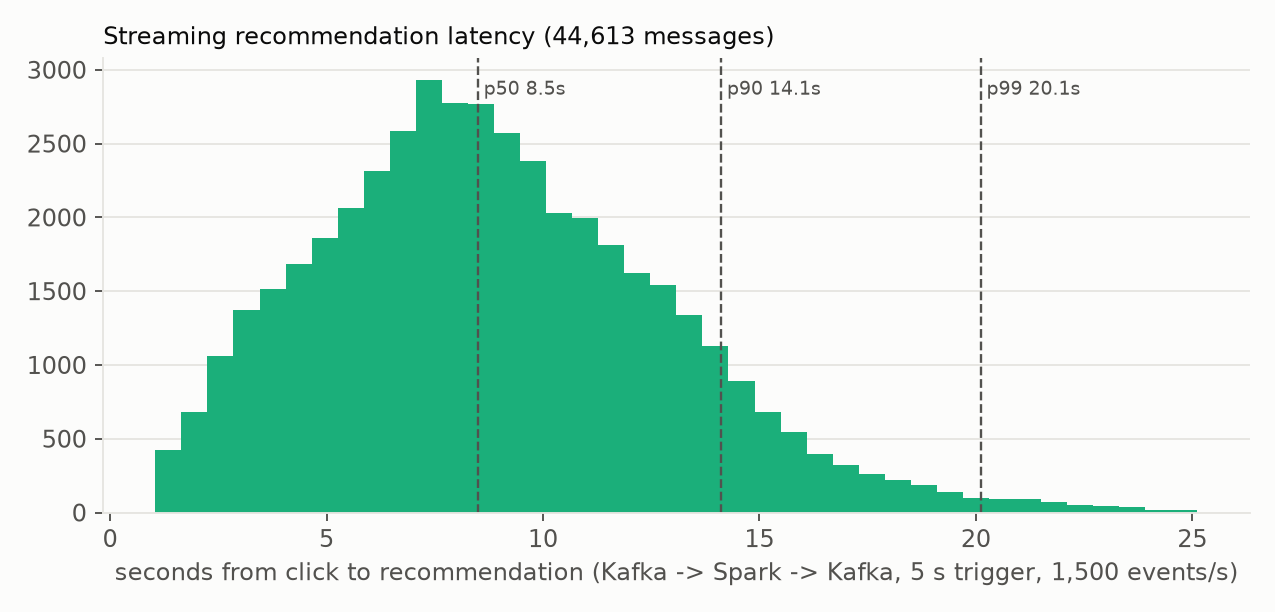
\includegraphics[width=0.88\columnwidth]{stream_latency.png}
\caption{Distribution of click-to-recommendation latency (44{,}613 messages).}
\label{fig:lat}
\end{figure}

\subsection{Tuning Benchmarks}
Table~\ref{tab:tuning} and Fig.~\ref{fig:tuning} report the measurements. Columnar storage and partition pruning dominate: a Parquet scan takes 1.1\,s versus 8.8\,s for the same rows as JSON, and one day of purchases takes 0.11\,s versus 1.84\,s for all 61 days. Eight files are read in 0.23\,s versus 1.52\,s for 500 small files, and writing takes 2.6\,s versus 15.0\,s. A broadcast join takes 1.1\,s versus 3.1\,s for sort-merge. With 24 shuffle partitions the aggregation takes 3.1\,s, against 12.6\,s with 400. Caching does not help for the three-query workload: it takes 14.8\,s including cache fill versus 5.6\,s uncached, and pays off only on re-use (3.9\,s warm). A Hadoop Streaming MapReduce job (shell/awk) that counts events per type over ten shards (10{,}484{,}105 records, 20 map tasks) returns counts identical to Spark.

\begin{table}[!t]
\caption{Tuning benchmarks (seconds, single runs)}
\label{tab:tuning}
\centering
\footnotesize
\begin{tabular}{@{}p{1.9cm}p{3.0cm}p{3.0cm}@{}}
\hline
\textbf{Exp.} & \textbf{Variant A} & \textbf{Variant B}\\\hline
E1 scan & JSON 8.79 & Parquet 1.14\\
E2 shuffle partitions & 4: 3.75; 24: 3.09 & 96: 4.31; 400: 12.61\\
E3 caching & none 5.63 & cache+fill 14.79; warm 3.87\\
E4 small files & write 500: 15.01; read 1.52 & write 8: 2.55; read 0.23\\
E5 join & sort-merge 3.14 & broadcast 1.14\\
E6 pruning & 61 days 1.84 & 1 day 0.11\\\hline
\end{tabular}
\end{table}

\begin{figure*}[!t]
\centering
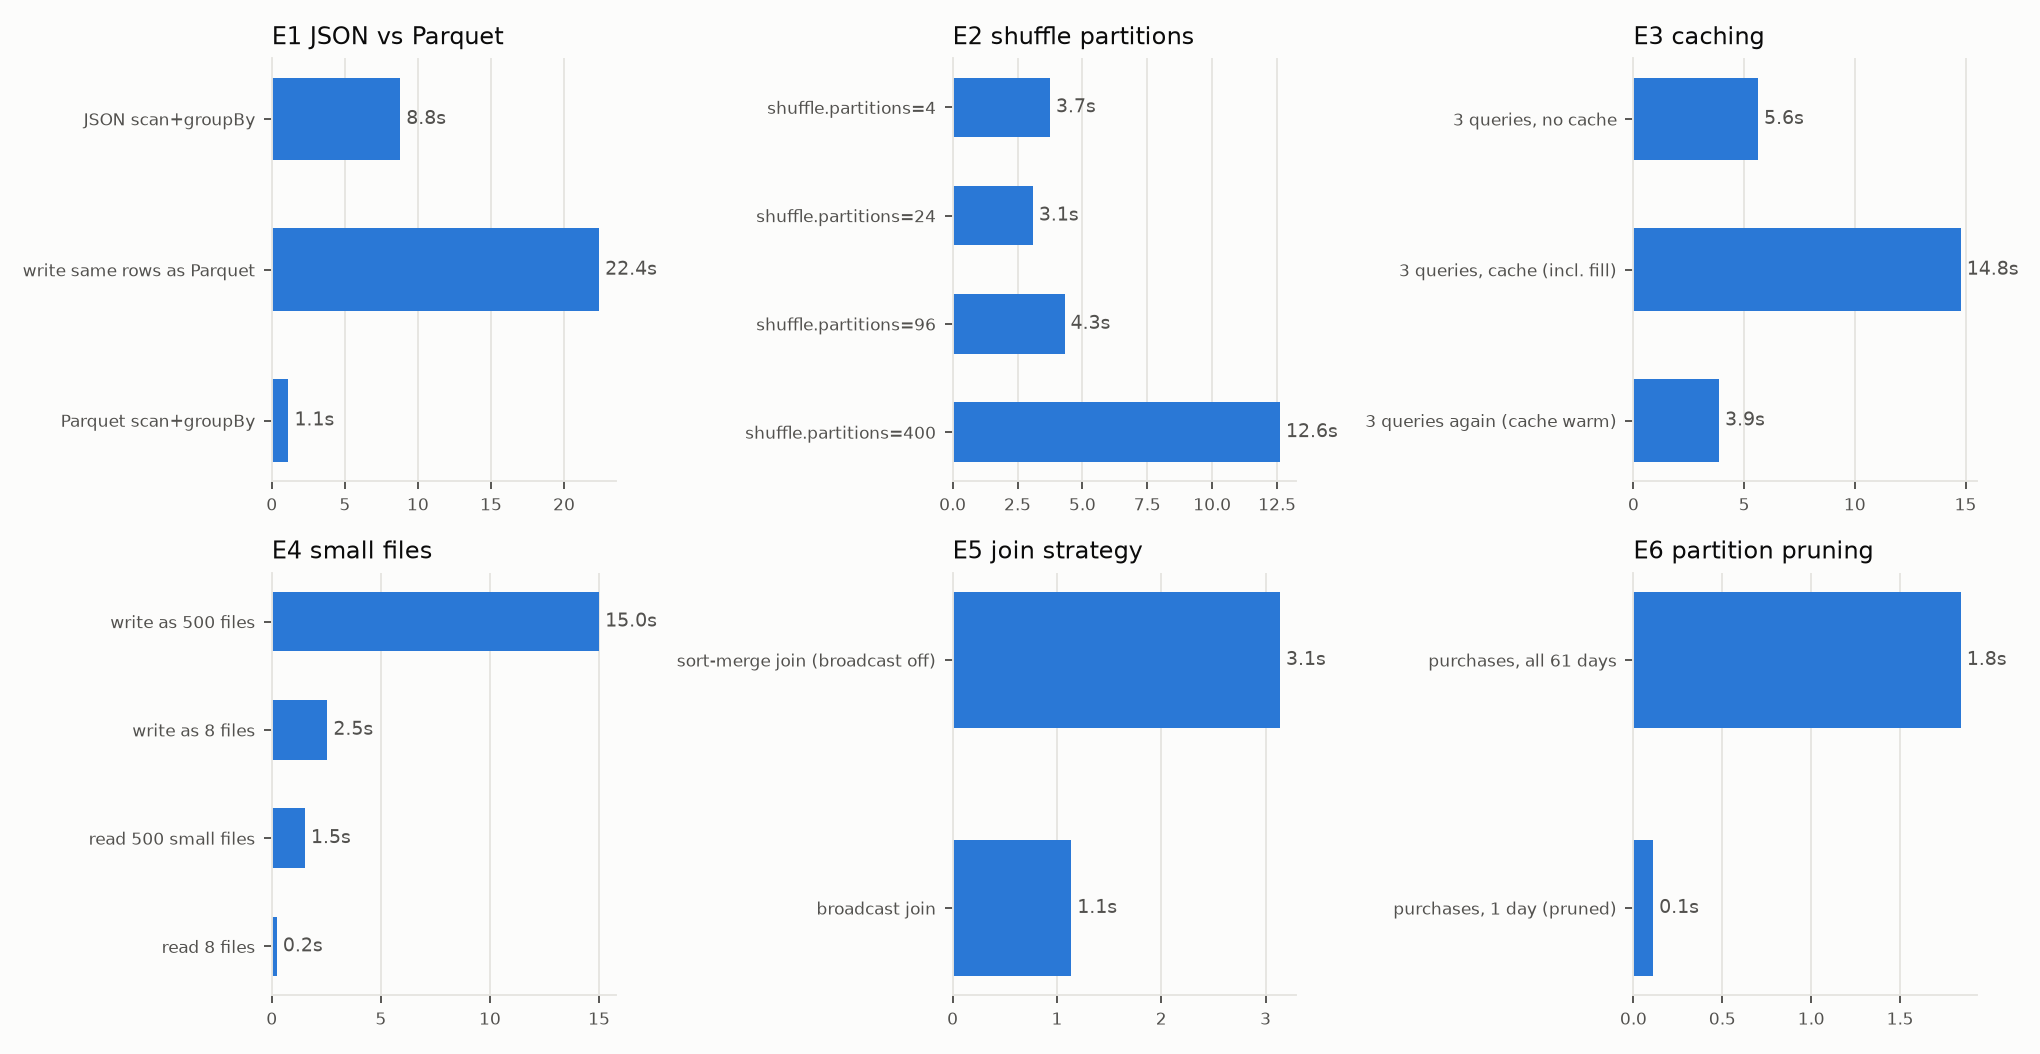
\includegraphics[width=0.68\textwidth]{tuning.png}
\caption{Tuning benchmark results E1--E6 (each run once).}
\label{fig:tuning}
\end{figure*}

\section{Discussion}
\textbf{Co-occurrence versus ALS.} The result that a simple item-to-item method outperforms both ALS variants is consistent with the finding of \cite{ludewig2021} that neighbour heuristics are often preferable to complex models in session-based settings. The following explanations are plausible but were not tested here. First, next-click behaviour within a session is dominated by local item-to-item transitions, which co-occurrence models directly, whereas ALS factorises an aggregated user--item matrix in which sequence is absent. Second, a session vector solved from one to three clicks is weakly constrained, and its quality depends on the factor rank and the confidence weighting. Third, the decline of fold-in accuracy with longer prefixes suggests that the first-event weights or popularity effects in the latent space influence the solution; ablations are required. For practice, the results indicate that a neighbour-style recommender is a strong, cheap first choice, and that fold-in is mainly attractive where an existing ALS model must be made session-aware without new infrastructure; the hybrid suggests that the two signals are partly complementary at the first click.

\textbf{Latency.} The fold-in computation (about 6\,ms) is small compared with the observed median of 8.5\,s, which is dominated by micro-batch scheduling, the 5\,s trigger and the Kafka hops. Shorter triggers or continuous processing would reduce the latency but were not evaluated, and page-level personalisation with sub-100\,ms budgets would call for serving fold-in from an in-memory service rather than from micro-batches. The reported latencies come from a single-NodeManager cluster and will differ on production hardware.

\textbf{Limitations.}
\begin{itemize}
\item Neural recommenders and the full SKNN family are not included, so conclusions about them cannot be drawn.
\item Each configuration is run once and no confidence intervals or significance tests are computed \cite{vinagre2021eval}; small differences, such as hybrid versus co-occurrence, are not established.
\item Evaluation uses 25\% of users and 20\% of test sessions, and the catalogue is limited to 45{,}863 of 206{,}876 products, so cold-start items are not evaluated.
\item User profiles and inventory are synthetic and event velocity is simulated by replay; the effect of relational features on recommendation quality is therefore not measured.
\item All three DataNodes share one disk, and the cluster has a single NodeManager with 1.25\,GB executors.
\end{itemize}

\section{Conclusion}
This paper presented a distributed streaming implementation of ALS fold-in with Kafka and Spark Structured Streaming on a Hadoop cluster and evaluated it on 110\,M real click events. Fold-in makes ALS session-aware at a cost of about 6\,ms per request and improves hit rate at 20 by a factor of 2.8 over stale batch ALS, but a simple item co-occurrence method remains the strongest single recommender, and a rank-fusion hybrid helps only at the first click. The streaming pipeline delivers recommendations with a median latency of 8.5\,s on commodity hardware, and the tuning measurements quantify the benefit of columnar storage, partition pruning and broadcast joins. The results suggest that, for streaming session recommendation, strong neighbour-style baselines should accompany any latent-factor method. Future work includes full SKNN and neural baselines (e.g., GRU4Rec) on GPU hardware, prequential evaluation with significance testing \cite{vinagre2021eval}, distributed hyper-parameter search, seeding fold-in with long-term user vectors, a multi-broker Kafka deployment and online experiments.

\appendices
\section{Configuration and Commands}
\textbf{Machine.} Intel i7-13620H, 15.7\,GB usable RAM, no usable GPU, Windows 11; WSL2 with \texttt{memory=12GB}, \texttt{processors=8}, \texttt{swap=4GB}.

\textbf{HDFS and YARN.} Replication 3, block size 128\,MB; YARN scheduler with 256\,MB minimum and 2048\,MB maximum allocation; NodeManager 3584\,MB and 6 vcores; virtual- and physical-memory checks disabled.

\textbf{Spark.} Spark 3.5.1, Scala 2.12.18, Java 8, adaptive execution on, Kryo serializer, \texttt{spark.yarn.archive} on HDFS, 2 executors $\times$ 1280\,MB $\times$ 2 cores, driver 768\,MB; shuffle partitions 96 (cleaning), 48 (training) and 6 (streaming).

\textbf{Commands.} Jobs are submitted with \texttt{scripts/run\_job.sh Class key=value}; the full command sequence is in the repository README.

\begin{thebibliography}{99}
\bibitem{ludewig2021} M.~Ludewig, N.~Mauro, S.~Latifi, and D.~Jannach, ``Empirical analysis of session-based recommendation algorithms,'' \emph{User Model.\ User-Adapted Interact.}, vol.~31, pp.~149--181, 2021, doi: 10.1007/s11257-020-09277-1.
\bibitem{wang2021survey} S.~Wang, L.~Cao, Y.~Wang, Q.~Z.~Sheng, M.~A.~Orgun, and D.~Lian, ``A survey on session-based recommender systems,'' \emph{ACM Comput.\ Surv.}, vol.~54, no.~7, Art.~no.~154, 2021, doi: 10.1145/3465401.
\bibitem{jakomin2020simf} M.~Jakomin, Z.~Bosni\'c, and T.~Curk, ``Simultaneous incremental matrix factorization for streaming recommender systems,'' \emph{Expert Syst.\ Appl.}, vol.~160, Art.~no.~113685, 2020, doi: 10.1016/j.eswa.2020.113685.
\bibitem{vinagre2021eval} J.~Vinagre, A.~M.~Jorge, C.~Rocha, and J.~Gama, ``Statistically robust evaluation of stream-based recommender systems,'' \emph{IEEE Trans.\ Knowl.\ Data Eng.}, vol.~33, no.~7, p.~2971, 2021, doi: 10.1109/TKDE.2019.2960216.
\bibitem{ji2023leakage} Y.~Ji, A.~Sun, J.~Zhang, and C.~Li, ``A critical study on data leakage in recommender system offline evaluation,'' \emph{ACM Trans.\ Inf.\ Syst.}, vol.~41, no.~3, Art.~no.~75, 2023, doi: 10.1145/3569930.
\bibitem{raptis2023kafka} T.~P.~Raptis and A.~Passarella, ``A survey on networked data streaming with Apache Kafka,'' \emph{IEEE Access}, 2023, doi: 10.1109/ACCESS.2023.3303810.
\bibitem{zaharia2016spark} M.~Zaharia \emph{et al.}, ``Apache Spark: A unified engine for big data processing,'' \emph{Commun.\ ACM}, vol.~59, pp.~56--65, 2016, doi: 10.1145/2934664.
\bibitem{li2020als} J.~B.~Li, S.~Y.~Lin, Y.~H.~Hsu, and Y.~C.~Huang, ``An empirical study of alternating least squares collaborative filtering recommendation for MovieLens on Apache Hadoop and Spark,'' \emph{Int.\ J.\ Grid Util.\ Comput.}, vol.~11, no.~5, p.~674, 2020, doi: 10.1504/IJGUC.2020.110053.
\bibitem{kumar2021edmfals} R.~R.~S.~Ravi~Kumar, G.~Appa~Rao, and S.~Anuradha, ``Efficient distributed matrix factorization alternating least squares (EDMFALS) for recommendation systems using Spark,'' \emph{J.\ Inf.\ Knowl.\ Manag.}, vol.~21, no.~1, Art.~no.~2250012, 2021, doi: 10.1142/S0219649222500125.
\bibitem{kechinov} M.~Kechinov, ``eCommerce behavior data from multi-category store,'' REES46 Open CDP, Kaggle dataset \url{mkechinov/ecommerce-behavior-data-from-multi-category-store}.
\end{thebibliography}

\end{document}
